%%
%% This is file `tikzposter-template.tex',
%% generated with the docstrip utility.
%%
%% The original source files were:
%%
%% tikzposter.dtx  (with options: `tikzposter-template.tex')
%%
%% This is a generated file.
%%
%% Copyright (C) 2014 by Pascal Richter, Elena Botoeva, Richard Barnard, and Dirk Surmann
%%
%% This file may be distributed and/or modified under the
%% conditions of the LaTeX Project Public License, either
%% version 2.0 of this license or (at your option) any later
%% version. The latest version of this license is in:
%%
%% http://www.latex-project.org/lppl.txt
%%
%% and version 2.0 or later is part of all distributions of
%% LaTeX version 2013/12/01 or later.
%%


\documentclass{tikzposter} %Options for format can be included here

\usepackage{todonotes}

\usepackage[tikz]{bclogo}
\usepackage{lipsum}
\usepackage{amsmath}


\usepackage{diagbox} %加载 diagbox 宏包之后可以绘制斜线表头
\usepackage{multirow} %加载 multirow 宏包后可以让表格单元实现合并与分割
\usepackage{makecell} %加载 makecell 宏包可以在表项中使用"\\"命令自由的换行。在不打算固定表列宽度时,它比p{宽度}选项更为灵活。


\usepackage{graphicx}
\usepackage{epstopdf}
\usepackage{subfigure}

\usepackage{booktabs}
\usepackage{longtable}
\usepackage[absolute]{textpos}
\usepackage[it]{subfigure}
\usepackage{graphicx}
\usepackage{cmbright}
%\usepackage[default]{cantarell}
%\usepackage{avant}
%\usepackage[math]{iwona}
\usepackage[math]{kurier}
\usepackage[T1]{fontenc}


%% add your packages here
\usepackage{hyperref}
% for random text
\usepackage{lipsum}
\usepackage[english]{babel}
\usepackage[pangram]{blindtext}

\colorlet{backgroundcolor}{blue!10}

 % Title, Author, Institute
 \title{New York City Taxi Fare Prediction}
 \author{Runsha Pan$^1$}
 \institute{$^1$ Hunan University, China 
 }
%\titlegraphic{logos/tulip-logo.eps}

%Choose Layout
\usetheme{Wave}

%\definebackgroundstyle{samplebackgroundstyle}{
%\draw[inner sep=0pt, line width=0pt, color=red, fill=backgroundcolor!30!black]
%(bottomleft) rectangle (topright);
%}
%
%\colorlet{backgroundcolor}{blue!10}

\begin{document}


\colorlet{blocktitlebgcolor}{blue!23}

 % Title block with title, author, logo, etc.
\maketitle

\begin{columns}
 % FIRST column
\column{0.5}% Width set relative to text width

%%%%%%%%%% -------------------------------------------------------------------- %%%%%%%%%%
 %\block{Main Objectives}{
%  	      	\begin{enumerate}
%  	      	\item Formalise research problem by extending \emph{outlying aspects mining}
%  	      	\item Proposed \emph{GOAM} algorithm is to solve research problem
%  	      	\item Utilise pruning strategies to reduce time complexity
%  	      	\end{enumerate}
%%  	      \end{minipage}
%}
%%%%%%%%%% -------------------------------------------------------------------- %%%%%%%%%%


%%%%%%%%%% -------------------------------------------------------------------- %%%%%%%%%%
\block{Introduction}{
  In this kaggle topic selection competition, you have to predict the taxi fare according to the known features of the passen-
  gers taking taxis, which including longitude coordinate and latitude co-
  ordinate of where the taxi ride started and so on. While you can get a basic estimate based on just the distance between the two points, this will result in an RMSE of $5-$8, the challenge is to do better than this using Machine Learning techniques!
  	
  \begin{description}
  	
    \item[Date files]
    The competition gives three documents train.csv, test.csv, sample\_submission.csv.
  	
  	\item[Data fields] 
    There are six features in the test and training sets,which includes "pickup\_datetime", "pickup\_longitude", "pickup\_latitude", "dropoff\_longitude", "dropoff\_latitude", "passenger\_count".

    \item[The Target]
    The target is predict "fare\_amount " field in "test.csv" file.
  \end{description}

  
}
%%%%%%%%%% -------------------------------------------------------------------- %%%%%%%%%%


%%%%%%%%%% -------------------------------------------------------------------- %%%%%%%%%%
\block{The evaluation metric}{
\begin{itemize}
    \item
    %\emph{Group Outlying Aspects Mining}
    The evaluation metric for this competition is the root mean-squared error or RMSE. RMSE measures the difference between the predictions of a model, and the corresponding ground truth. A large RMSE is equivalent to a large average error, so smaller values of RMSE are better. One nice property of RMSE is that the error is given in the units being measured, so you can tell very directly how incorrect the model might be on unseen data.
    % It aims to \emph{identify a subset of aspects (or subspace)
    % which makes the query group, rather than the single object,
    % obviously different}.
    % What we are interested in the task of \emph{group outlying aspects mining}
    % is to explain which aspects make the query group distinctive
    % different from the other groups.

    \item
    RMSE is given by:$$
{RMSE =\sqrt{\frac{1}{n}\sum_{i=1}^n (\hat{y_i}-y_i)^2}}
$$where $y_i$ is the ith observation and $\hat{y_i}$ is the prediction for that observation.
    % \emph{Group Outlying Aspects Mining},
    % \emph{Outlying Aspects Mining} and
    % \emph{Outlier Detection} are different with each other.
\end{itemize}

% \begin{center}
%     \begin{minipage}{0.3\linewidth}
%     \centering
%     \begin{tikzfigure}
%     \missingfigure[figcolor=white]{Testing figcolor}
%     {\small{Group Outlying Aspects Mining}}
%     \end{tikzfigure}%
%     \end{minipage}
%     \hfill
%     \begin{minipage}{0.3\linewidth}
%     \centering
%     \begin{tikzfigure}
%     \missingfigure[figcolor=white]{Testing figcolor}
%     {\small{Outlying Aspects Mining}}
%     \end{tikzfigure}%
%     \end{minipage}
%     \hfill
%     \begin{minipage}{0.3\linewidth}
%     \centering
%     \begin{tikzfigure}
%     \missingfigure[figcolor=white]{Testing figcolor}
%     {\small{Outlier Detection}}
%     \end{tikzfigure}%
%     \end{minipage}
% \end{center}
}
%%%%%%%%%% -------------------------------------------------------------------- %%%%%%%%%%


%%%%%%%%%% -------------------------------------------------------------------- %%%%%%%%%%

%\note{Note with default behavior}

%\note[targetoffsetx=12cm, targetoffsety=-1cm, angle=20, rotate=25]
%{Note \\ offset and rotated}

 % First column - second block


%%%%%%%%%% -------------------------------------------------------------------- %%%%%%%%%%
\block{Data viewing and preliminary analysis}{
  	% We propose the \emph{GOAM} algorithm to solve the research problem of
    % \emph{Group Outlying Aspects Mining}.
  	% The \emph{GOAM} algorithm includes three major steps.
%    1) Group Feature Extraction,
%    2) Outlying Degree Scoring, and
%    3) Outlying Aspects Identification.
  	
% \begin{tikzfigure}%[Overall architecture of \emph{GOAM} algorithm]
% %  \includegraphics[width=0.8\linewidth]{figures//framework.pdf}
%     \missingfigure[figcolor=white]{Testing figcolor}
% \end{tikzfigure}
		
\begin{description}
  	\item[Data Viewing]
  	The author analyzed the data through jupyter.Firstly, for the imported data, remove the first five rows of the training set and the test set to see the general situation of the data, and output the field and data type information.Among them, since the training set is too large and contains 5400W rows, the first 200W rows are selected for training in order to save running time. And calculate the number of data contained in the test set and the training set, the mean, variance, standard deviation, minimum value, maximum value, quartile and median, in order to understand the basic situation of the data, from which you can roughly understand the simple abnormal situation of the data.
    \item[Data Visualization]
    Combined with the data description results of the training set, the histogram of passenger consumption in the training set was made, and the outliers of passenger consumption were screened and removed.
\end{description}
    
    


    % \begin{figure}[htbp]
    %   \centering
    %   \subfigure[figure 1:100 groups]
    %   {
    %       \begin{minipage}[b]{.3\linewidth}
    %           \centering
    %           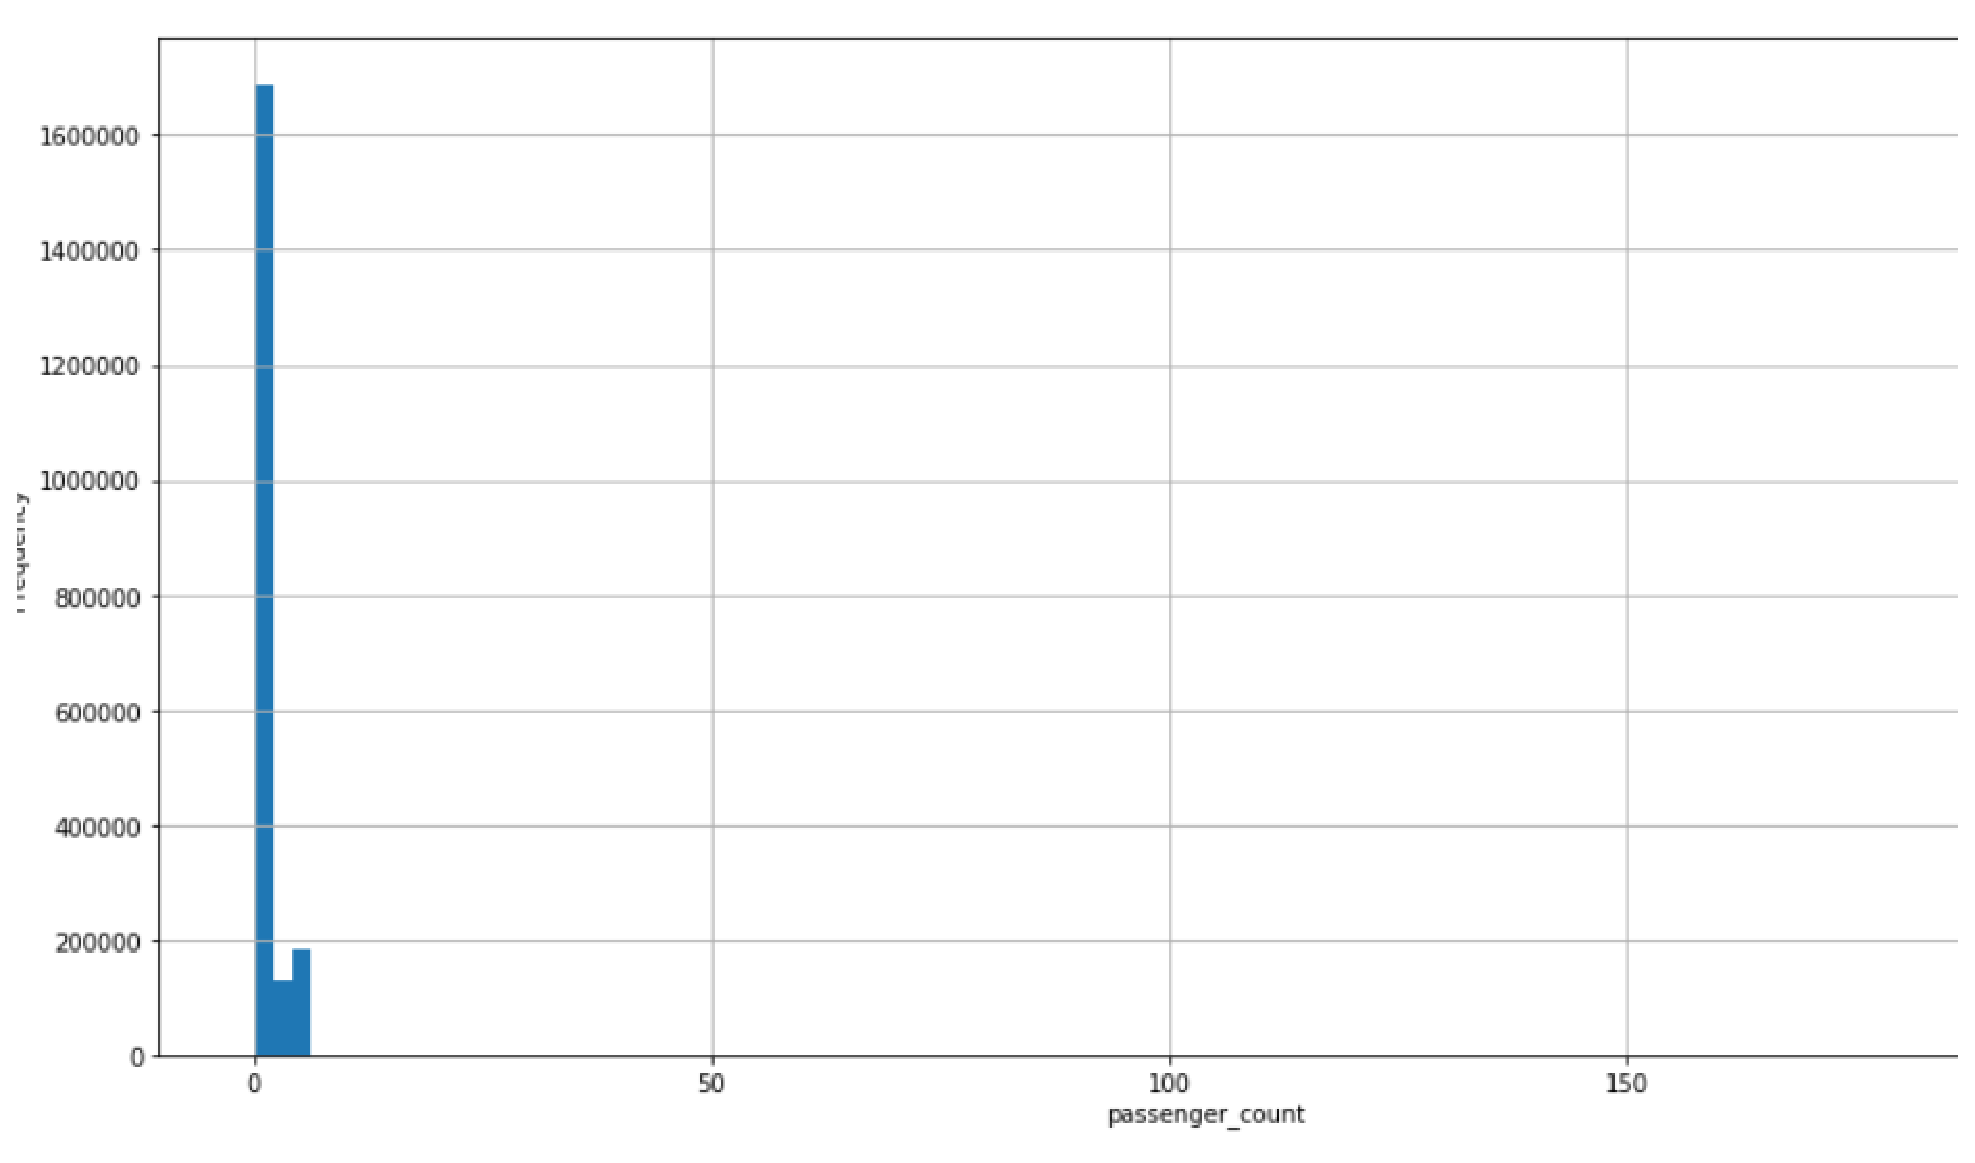
\includegraphics[height = 1.5cm, width = 3cm]{01.eps}
    %           \label{fig:fre-dis-f3}
    %       \end{minipage}
    %   }
    %   \subfigure[figure 2:10 groups,x<10]
    %   {
    %     \begin{minipage}[b]{.3\linewidth}
    %           \centering
    %           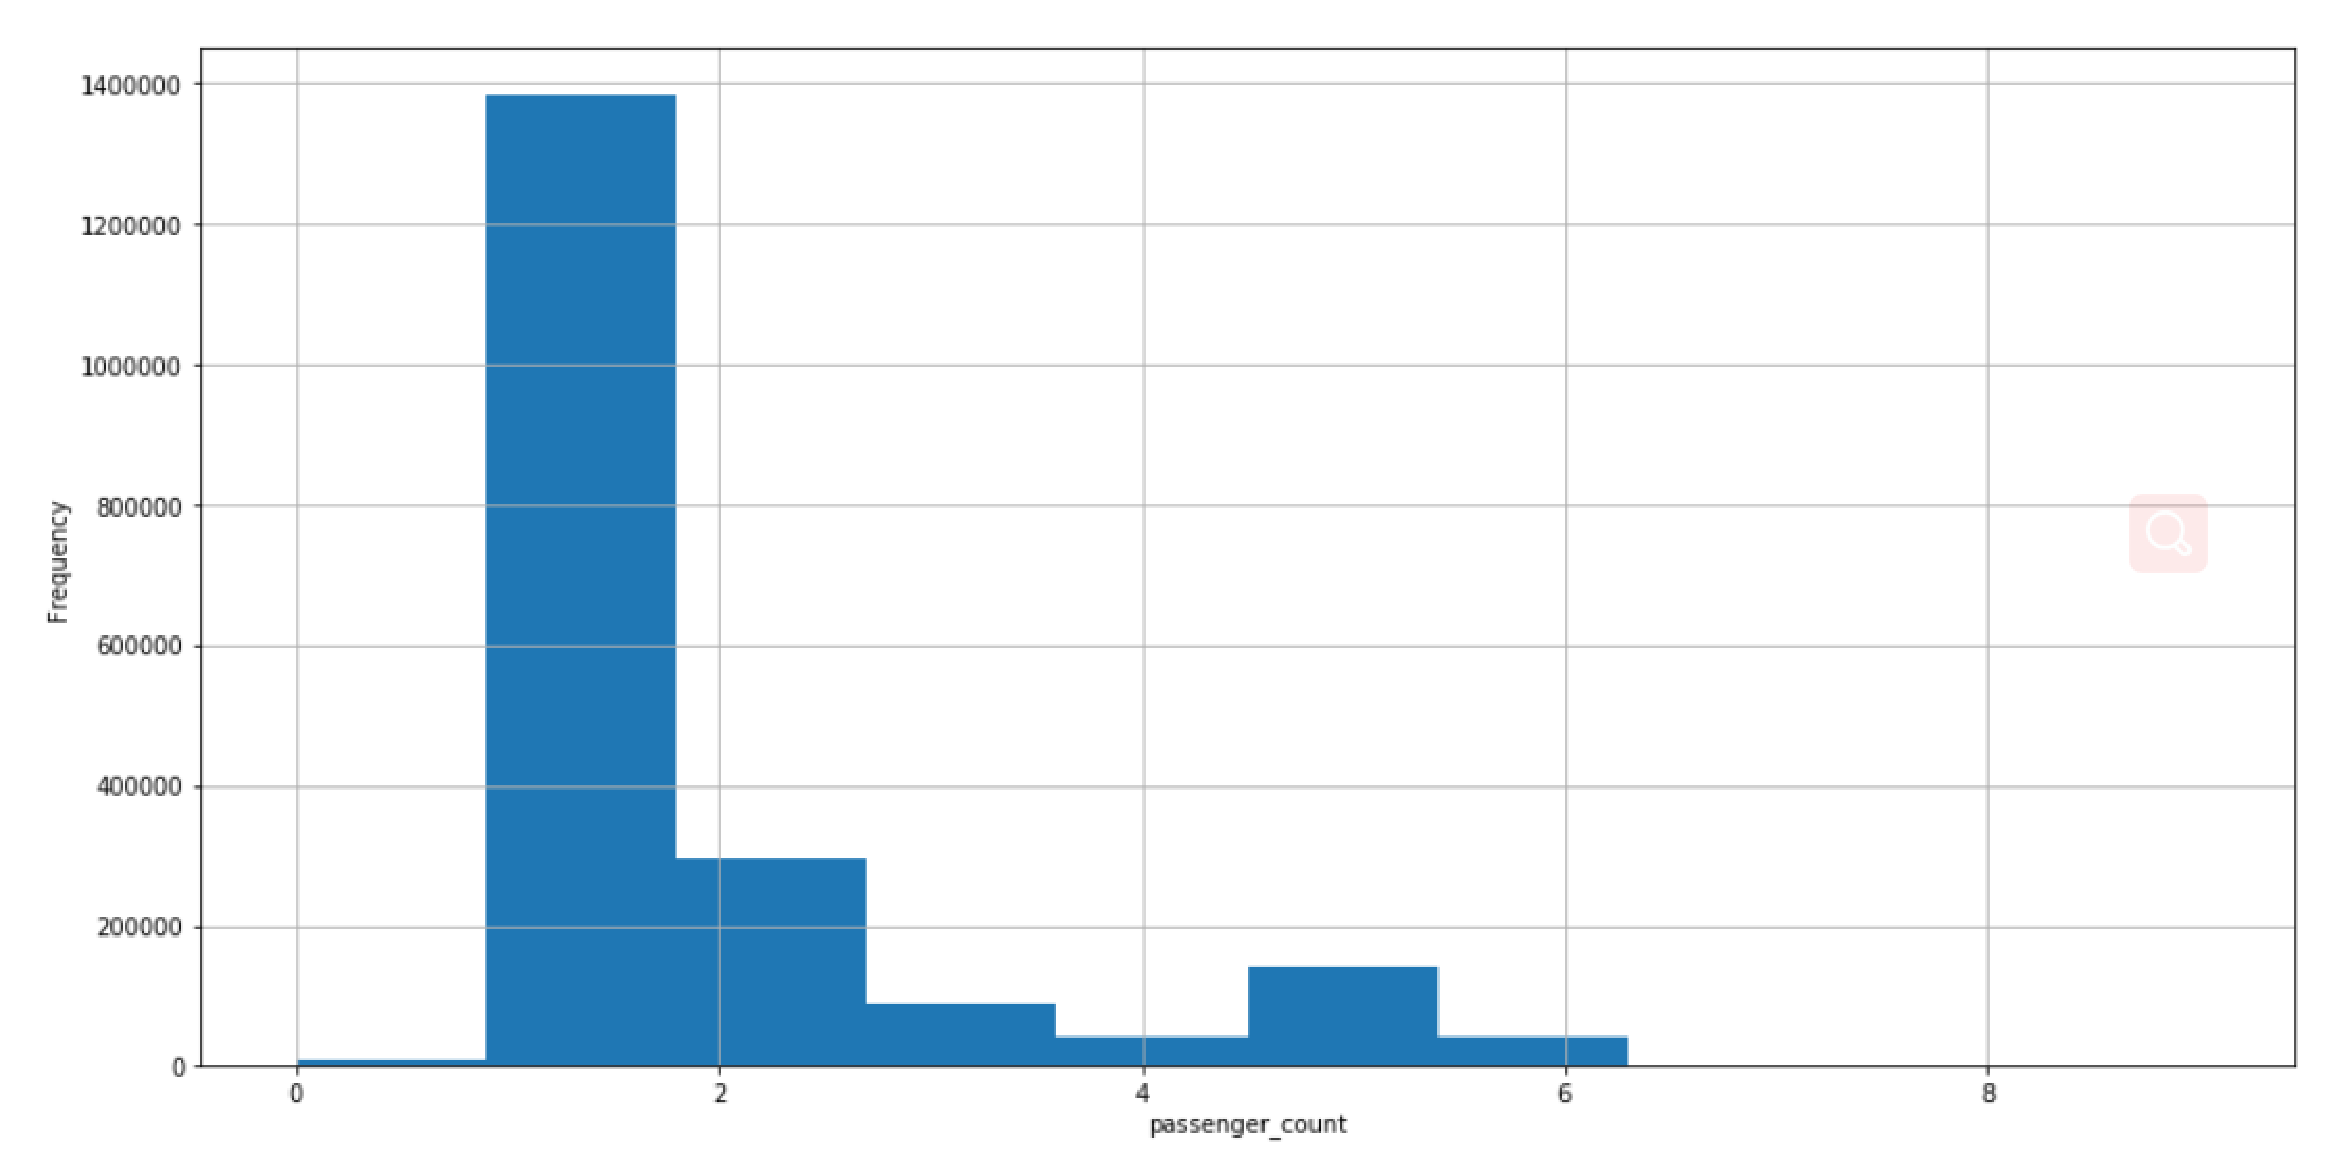
\includegraphics[height = 1.5cm, width = 3cm]{2.eps}
    %       \end{minipage}
    %   }
    %   \subfigure[figure 3:10 groups,x>=10]
    %   {
    %     \begin{minipage}[b]{.3\linewidth}
    %           \centering
    %           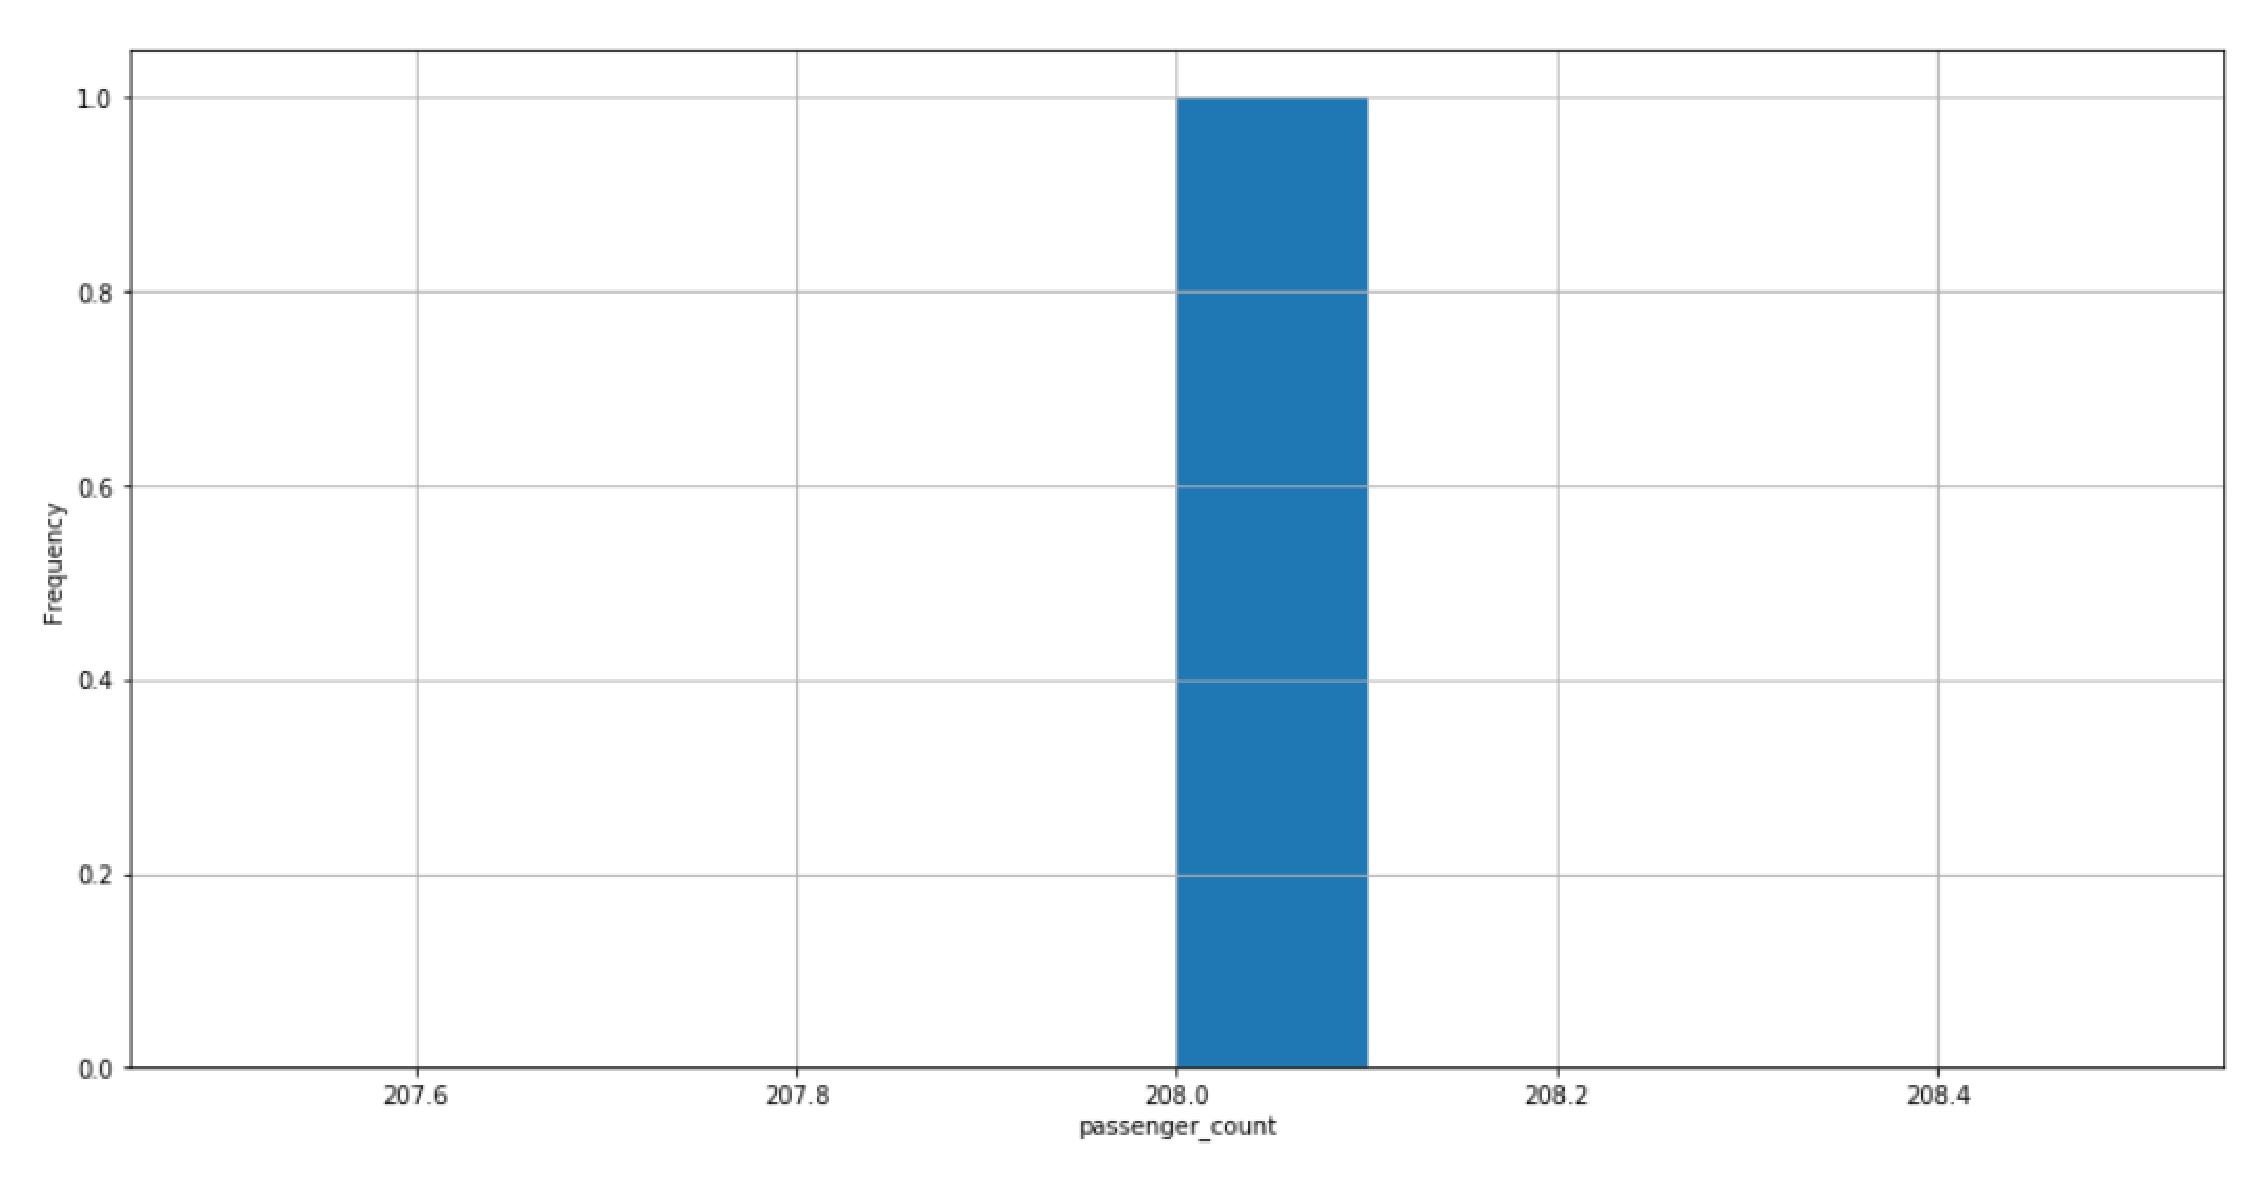
\includegraphics[height = 1.5cm, width = 3cm]{3.eps}
    %       \end{minipage}
    %   }
    %   \caption{Histogram of different groups}
    %   \end{figure}


    % Let $f_1$, $f_2$, $f_3$ represent three features of $G_q$.
    % We count the frequency of each value for one feature.
    % Then use the histogram to represent each feature.
    % Similarly,
    % we can extract other features for each group.
\bigskip
\begin{center}
      \begin{minipage}{0.3\linewidth}
      \centering
      \begin{tikzfigure}
      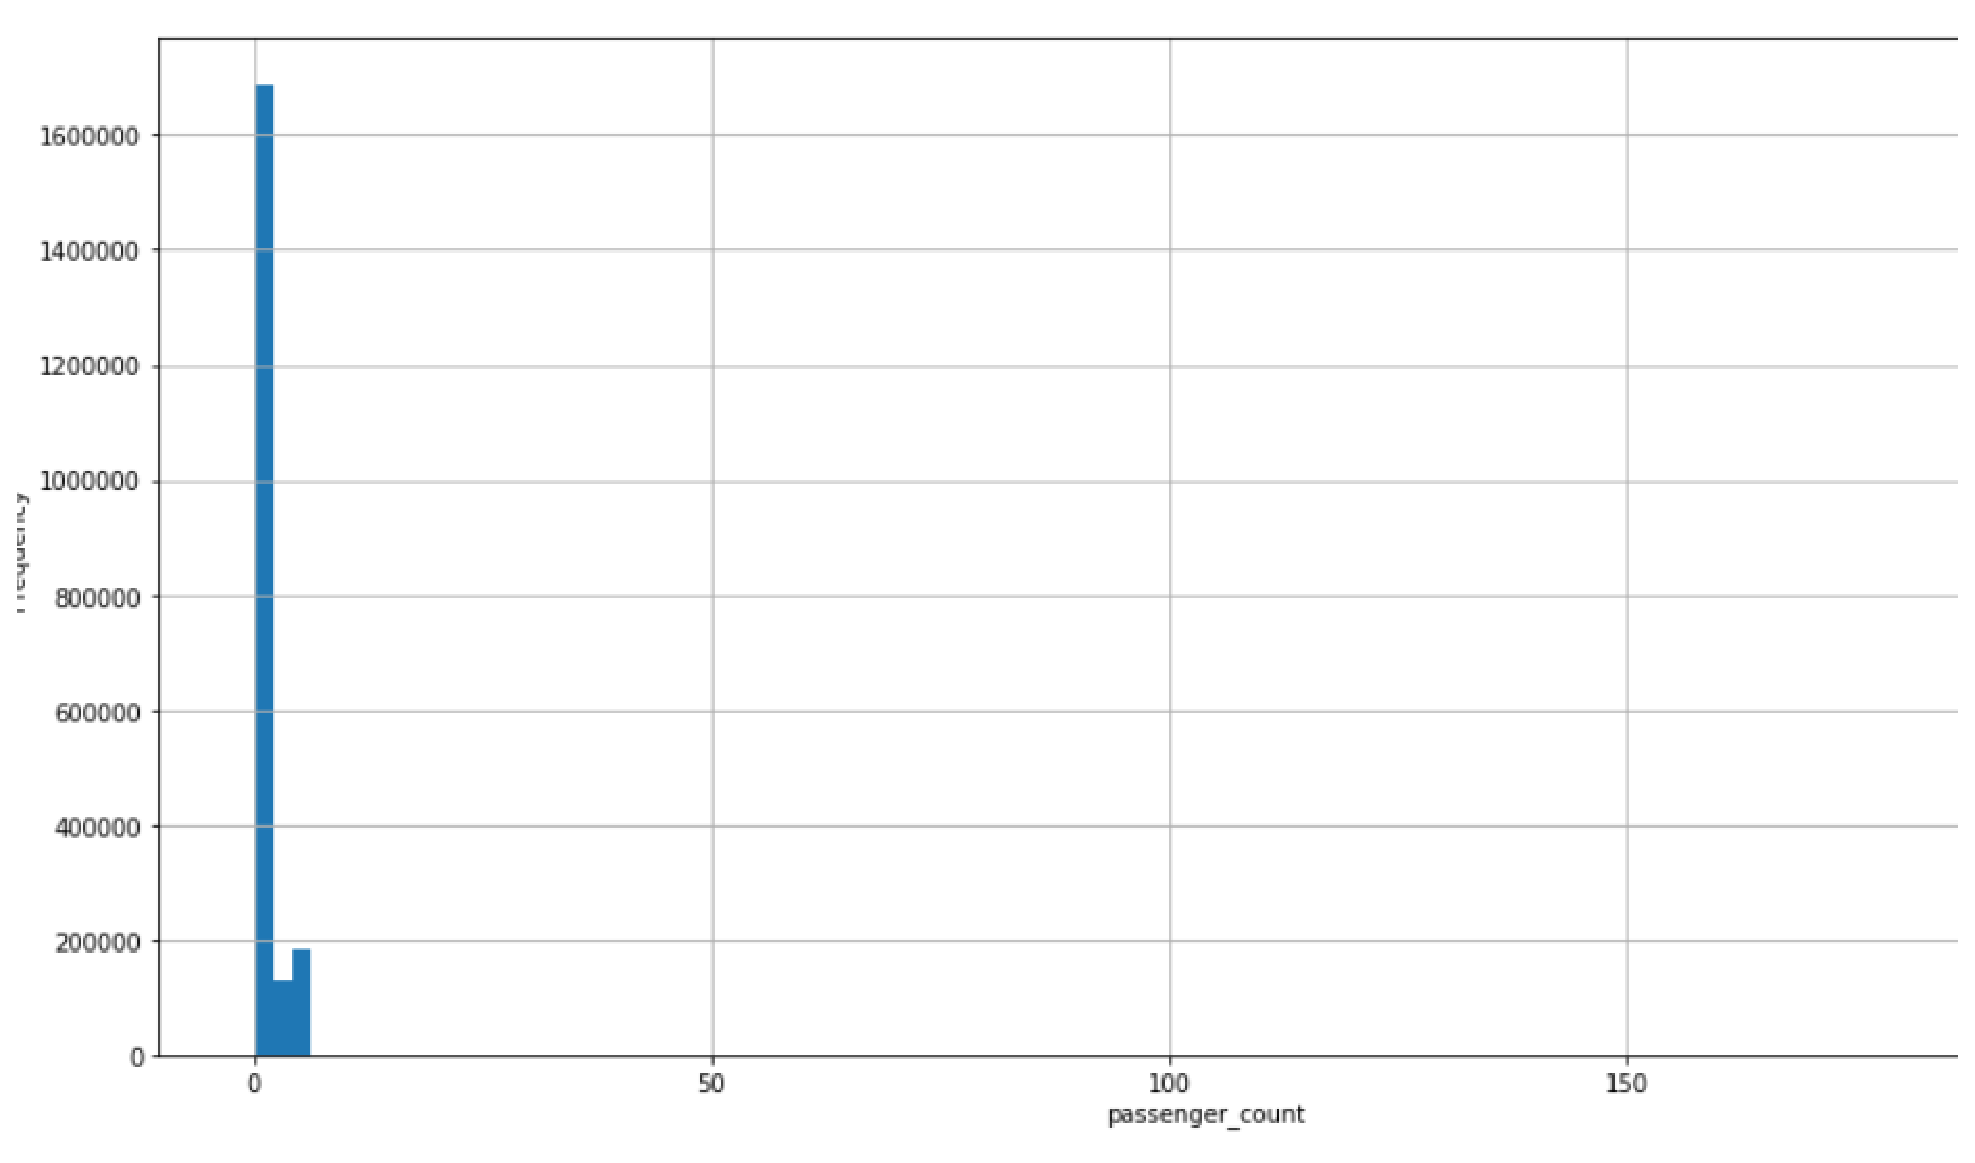
\includegraphics[height = 5cm, width = 10cm]{01.eps}  
        % \missingfigure[figcolor=white]{Testing figcolor}
      {\small{figure 1:100 groups}}
      \end{tikzfigure}%
      \end{minipage}
      \hfill
      \begin{minipage}{0.3\linewidth}
      \centering
      \begin{tikzfigure}
      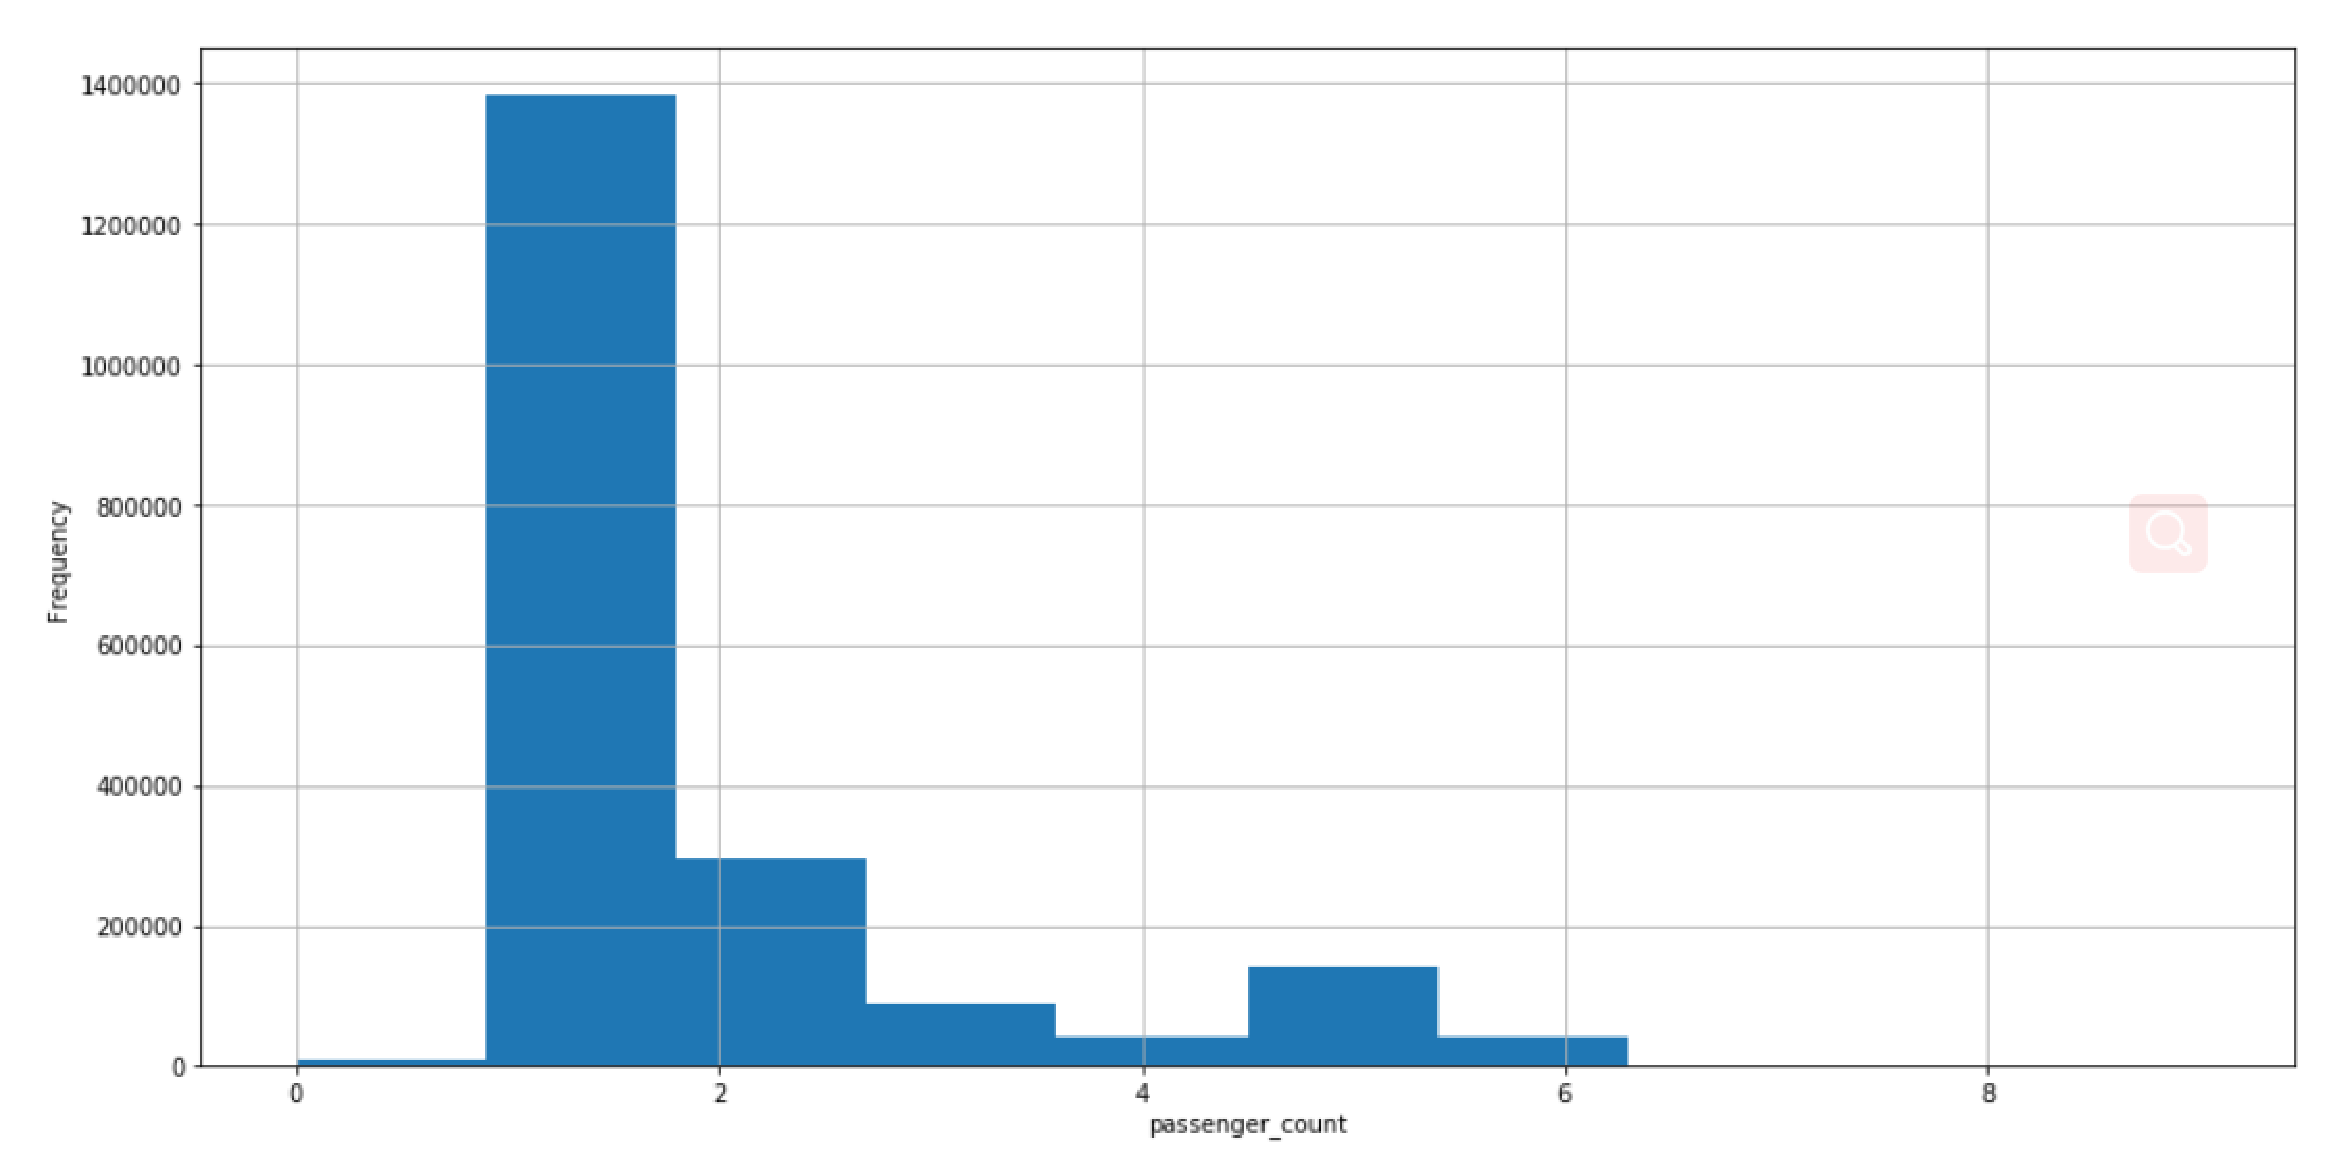
\includegraphics[height = 5cm, width = 10cm]{2.eps}
      % \missingfigure[figcolor=white]{Testing figcolor}
      {\small{figure 2:10 groups,x<10}}
      \end{tikzfigure}%
      \end{minipage}
      \hfill
      \begin{minipage}{0.3\linewidth}
      \centering
      \begin{tikzfigure}
      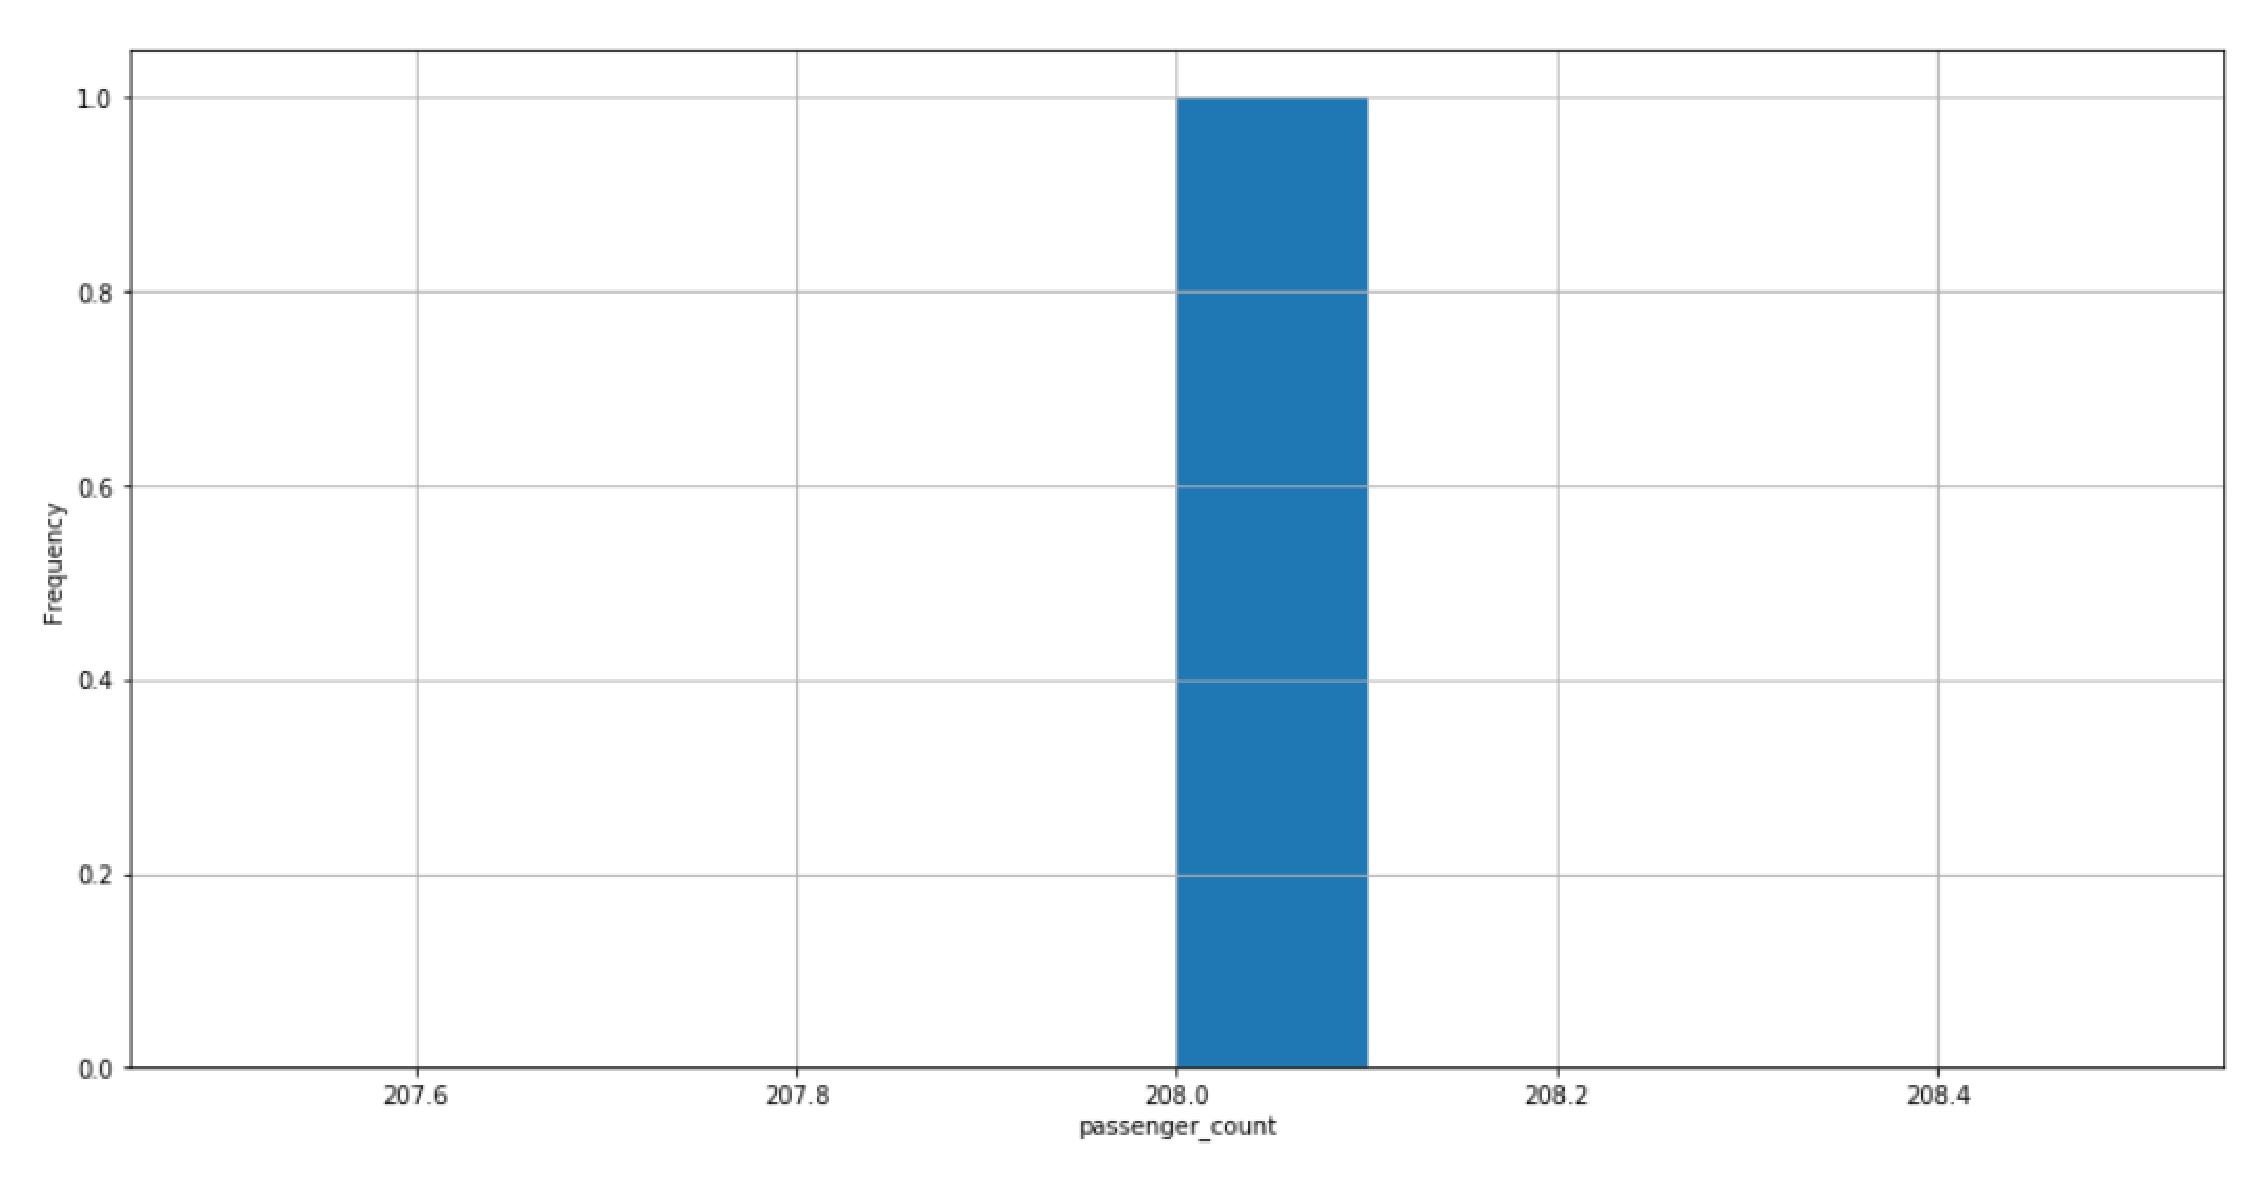
\includegraphics[height = 5cm, width = 10cm]{3.eps}
      % \missingfigure[figcolor=white]{Testing figcolor}
      {\small{figure 3:10 groups,x>=10}}
      \end{tikzfigure}%
      \end{minipage}
\end{center}
\bigskip

\begin{description}
    \item[Data Conversion]
    The timestamp data types in the training set and the test set were converted into numerical data that were easy to analyze and convenient for subsequent analysis.
    \item[Data Calculation]
    Exploring the data further. Firstly, 14 rows with missing values were deleted, resulting in 1999986 remaining rows. Secondly, handling outliers. Trim the rows with negative taxi fares, pick-up/drop-off longitude outside the range (-180-180), pick-up/drop-off latitude outside the range (-90-90).
%    \item
%    The histogram of $G_q$ on three features are as follows.
\end{description}

% \begin{center}
%   \begin{minipage}{0.3\linewidth}
%   \centering
%   \begin{tikzfigure}
%   % 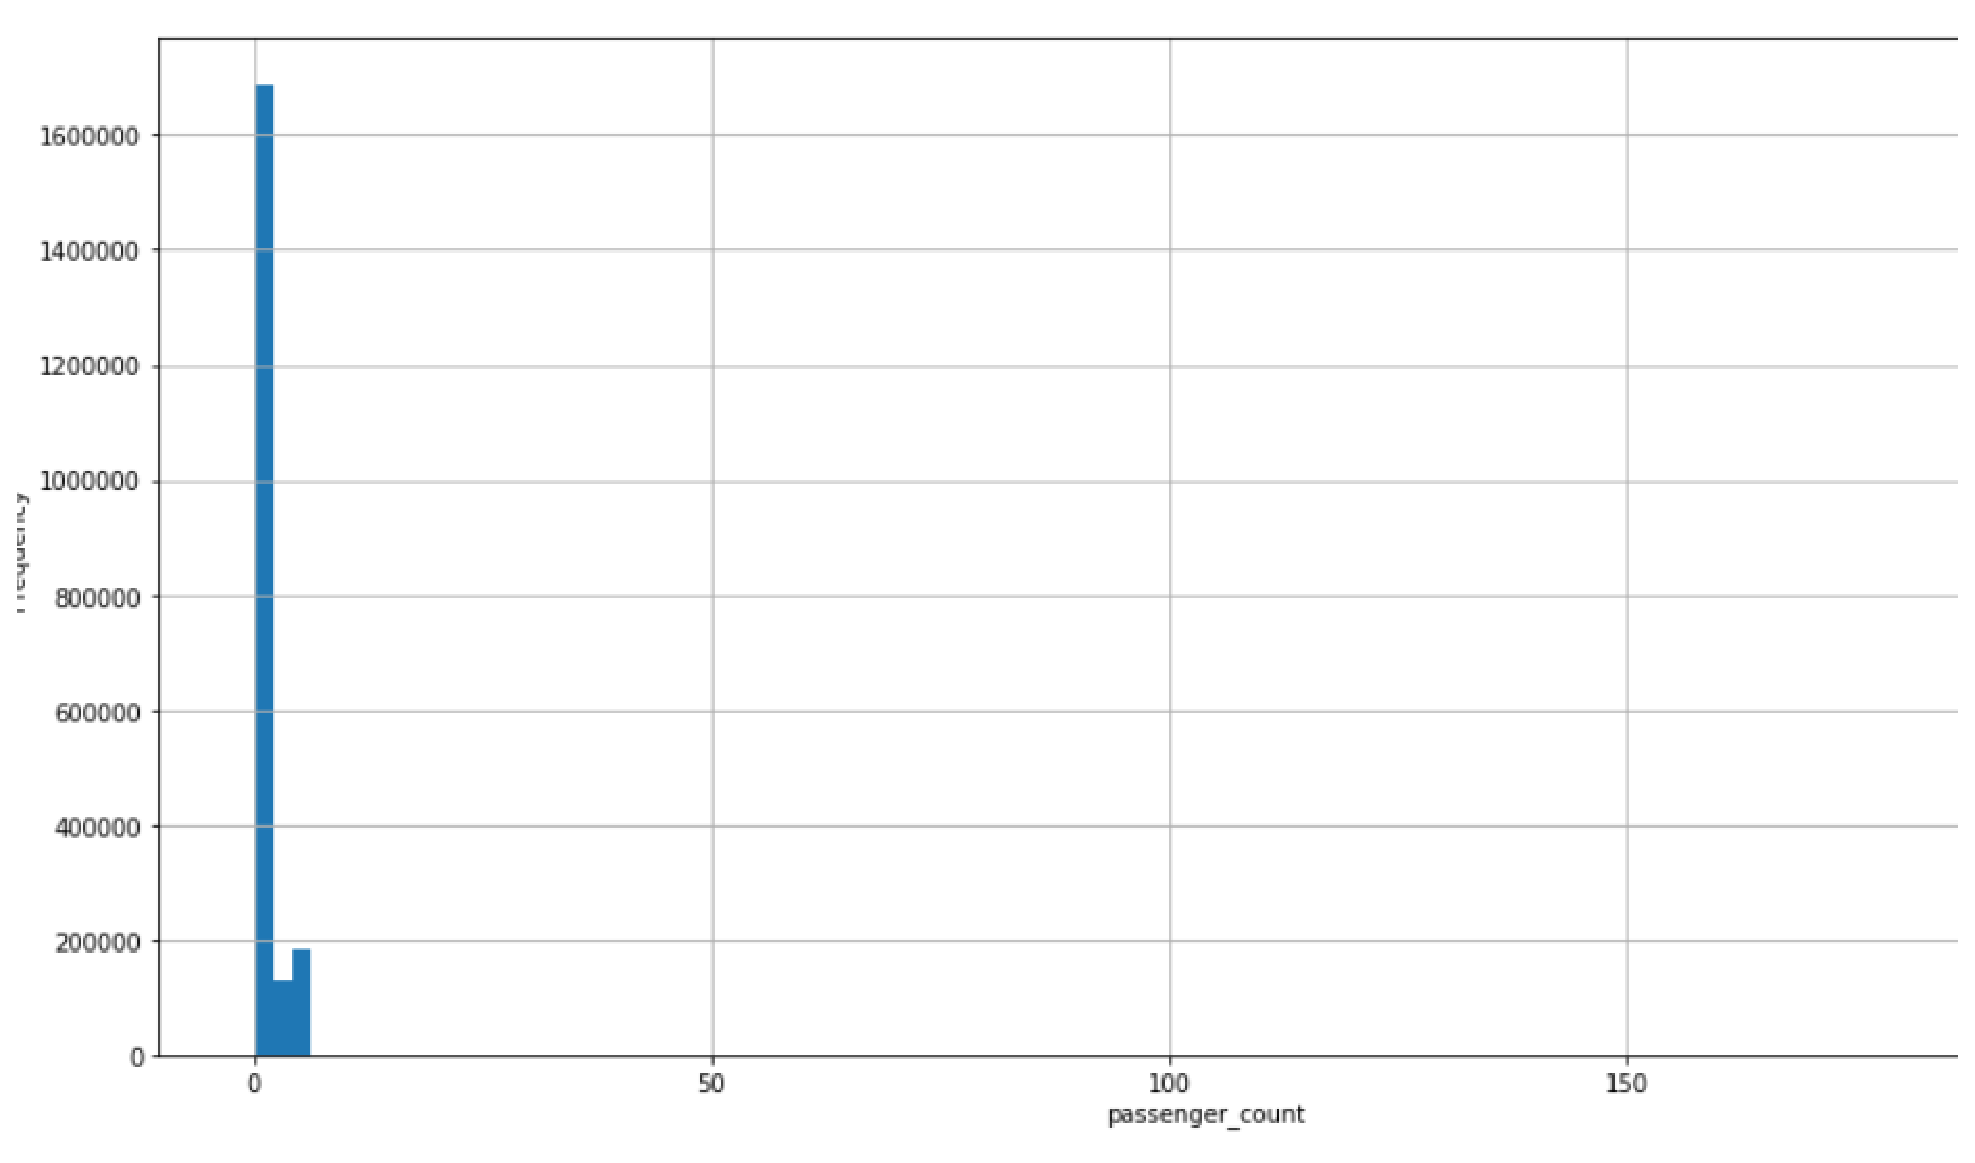
\includegraphics[height = 1.5cm, width = 3cm]{01.eps}
%   \missingfigure[figcolor=white]{Testing figcolor}
%   {\small{Group Outlying Aspects Mining}}
%   \end{tikzfigure}%
%   \end{minipage}
%   \hfill

%   \begin{minipage}{0.3\linewidth}
%   \centering
%   \begin{tikzfigure}
%   % 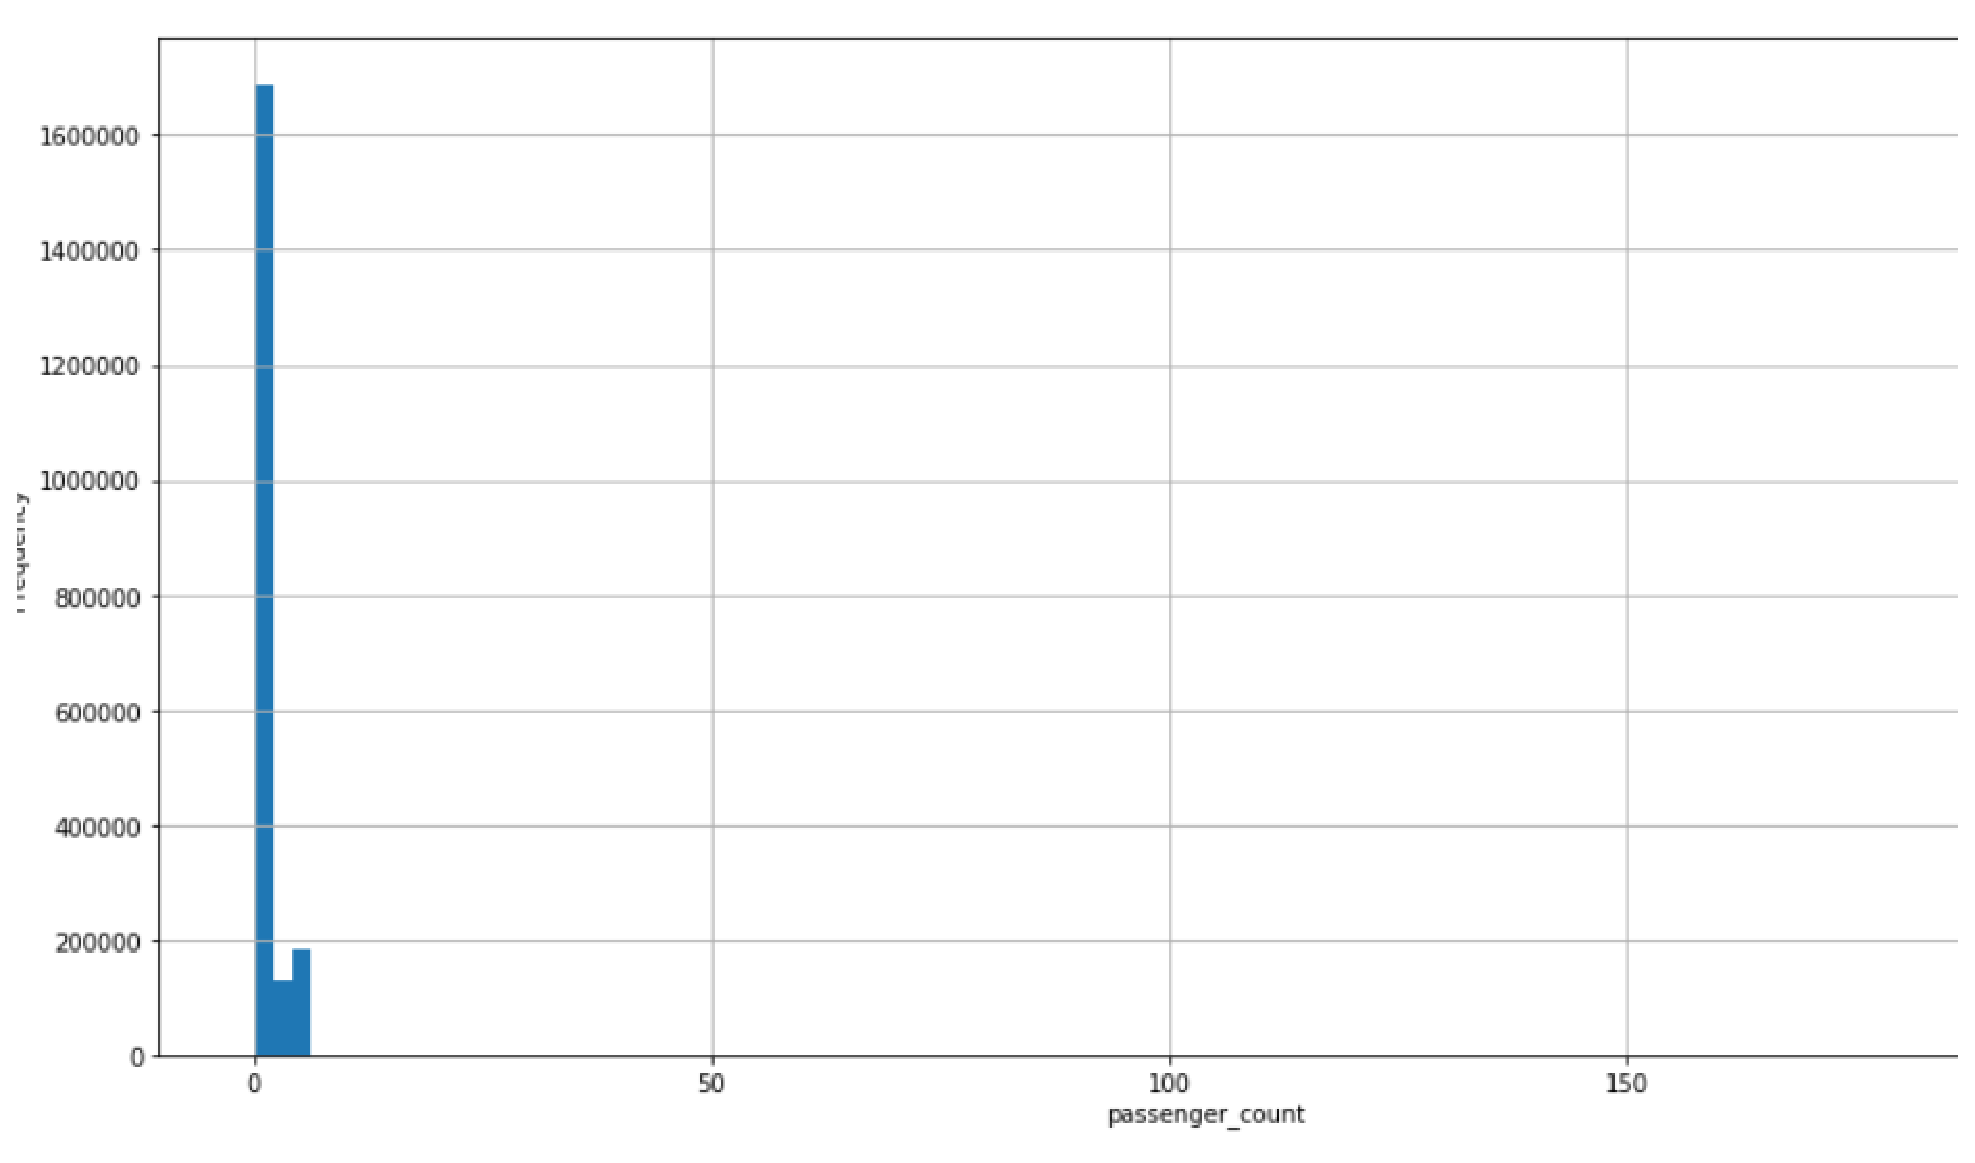
\includegraphics[height = 1.5cm, width = 3cm]{01.eps}
%   \missingfigure[figcolor=white]{Testing figcolor}
%   {\small{Outlying Aspects Mining}}
%   \end{tikzfigure}%
%   \end{minipage}
%   \hfill

%   \begin{minipage}{0.3\linewidth}
%   \centering
%   \begin{tikzfigure}
%   % 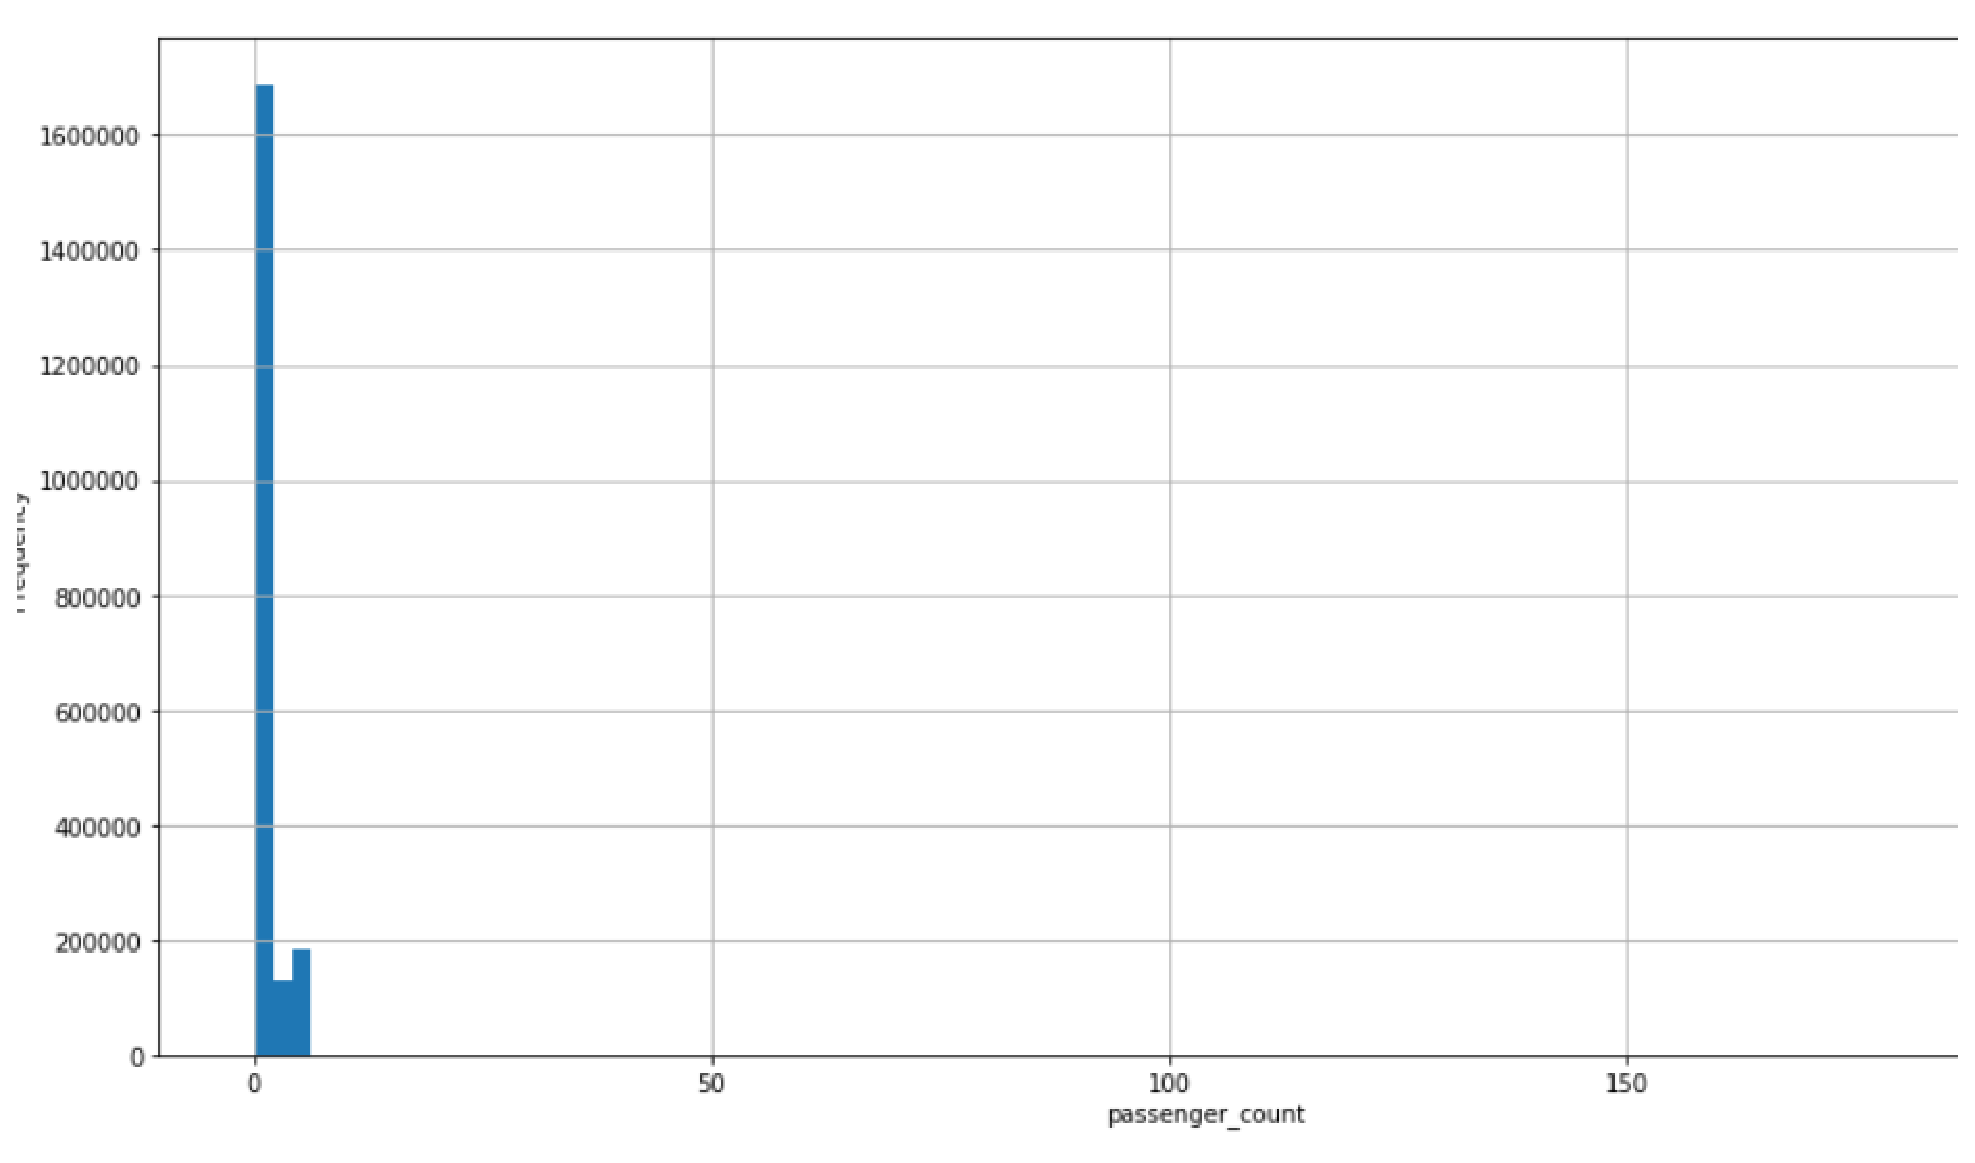
\includegraphics[height = 1.5cm, width = 3cm]{01.eps}
%   \missingfigure[figcolor=white]{Testing figcolor}
%   {\small{Outlier Detection}}
%   \end{tikzfigure}%
%   \end{minipage}
% \end{center}

% \begin{center}
%     \begin{minipage}{0.3\linewidth}
%     \centering
%     \begin{tikzfigure}
%     \missingfigure[figcolor=white]{Testing figcolor}
%     {\small{Histogram of $G_q$ on $f_1$}}
%     \end{tikzfigure}%
%     \end{minipage}
%     \hfill
%     \begin{minipage}{0.3\linewidth}
%     \centering
%     \begin{tikzfigure}
%     \missingfigure[figcolor=white]{Testing figcolor}
%     {\small{Histogram of $G_q$ on $f_2$}}
%     \end{tikzfigure}%
%     \end{minipage}
%     \hfill
%     \begin{minipage}{0.3\linewidth}
%     \centering
%     \begin{tikzfigure}
%     \missingfigure[figcolor=white]{Testing figcolor}
%     {\small{Histogram of $G_q$ on $f_3$}}
%     \end{tikzfigure}%
%     \end{minipage}
% \end{center}


% \begin{description}
% \item[Outlying Degree Scoring]
%     In this step,
%     we first calculate the \emph{earth mover distance} (EMD) of one feature among different groups.
%     The earth mover distance reflects the minimum mean distance
%     between groups on one feature.
%     So,
%     we utilize the EMD to measure the difference between groups of each feature.
% \end{description}
}
%%%%%%%%%% -------------------------------------------------------------------- %%%%%%%%%%


% SECOND column
\column{0.5}
 %Second column with first block's top edge aligned with with previous column's top.

%%%%%%%%%% -------------------------------------------------------------------- %%%%%%%%%%
\block{Data Reduction and computation}{
\begin{description}
    \item
    Through the histogram drawing, the outliers with the number of passengers greater than 10 are found, and a record is screened out for deletion.After pruning, 1999822 pieces of training set data were obtained.
    
    In order to make the data of the training set and the test set closer and simplify the training samples, the longitude and latitude range of the test set was found out, and the training set data was framed in this range to perform data pruning. 
    The post-construction training dataset contains 1957,917 records. 
\end{description}

% \begin{tikzfigure}%[Overall architecture of \emph{GOAM} algorithm]
%     \missingfigure[figcolor=white]{Testing figcolor}
% \end{tikzfigure}
%   where $G_q$ is the query group,
%   $n$ is the number of compare groups,
%   and $h_{k_s}$ is the histogram representation of $G_k$ in the subspace $s$.

\begin{description}
  	\item[Distance]
    the distance between the pick-up and drop-off locations of the training set and the test set was calculated according to the Haversine Equation, and a new field was formed and added to the data set. The records with zero distance between taxi fare and pick-up and drop-off location are invalid, and 1957913 training set data are obtained after deletion.
\end{description}
}
%%%%%%%%%% -------------------------------------------------------------------- %%%%%%%%%%
% Second column - first block


%%%%%%%%%% -------------------------------------------------------------------- %%%%%%%%%%
\block[titleleft]{Model Building}
{
\begin{description}
  	\item[Model] The expression of the multivariate linear regression model is$$
    {Y_i} ={\beta_0}+{\beta_1}{X_{0_i}}+{\beta_2}{X_{1_i}}+\cdots+{\beta_k}{X_{k_i}}+{\mu}
    $$where i=1, 2, ..., n.

    Matrix representation:$$
    {Y} ={X}{\beta}+{\mu}$$
    \item[Solution]
    In this paper, the pick-up and drop-off distance, travel time (day of the week), and the number of passengers are used as independent variables to construct matrix X for solving: 
    \begin{equation*}
      \left[
      \begin{array}{cccc}
      x_{0} &...  & x_{0}^{n} & 1\\
      x_{1} &...  & x_{1}^{n} & 1\\
        &...&  &\\
      x_{n} &...  &x_{n}^{n} & 1
      \end{array}
      \right ]
      \left[
      \begin{array}{cccc}
      {\beta}_{1}\\
      \ldots \\
      {\beta}_{n}\\
      {\beta}_{0}
      \end{array}
      \right ]
      =
      \left[
      \begin{array}{cccc}
      y_{0}\\
      y_{1}\\
      \ldots \\
      y_{n}
      \end{array}
      \right ]
    \end{equation*}
    
    It is solved using the least squares method:$$
    {\beta}=({X^T}{X})^{-1}{X^T}Y
    $$

    The multiple regression equation is obtained as follows:$$
    {Y_i} =4.46+2.10{X_{0_i}}-0.05{X_{1_i}}+0.04{X_{2_i}}
    $$where ${X_{0_i}}$ is the value of "H\_Distance", ${X_{1_i}}$ is the value of "weekday+1", ${X_{2_i}}$ is the value of "passenger\_count".


\end{description}
\vspace{.5cm}
% \begin{tabular}{ c | c | c | c }
%     \toprule
%     Method     &  Truth Outlying Aspects    & Identified Aspects & Accuracy      \\
%     \midrule
%     GOAM       &  $\{F_1\}$, $\{F_2F_4\}$   &  $\{F_1\}$, $\{F_2F_4\}$    & 100\%    \\

%      Arithmetic Mean based OAM &  $\{F_1\}$, $\{F_2F_4\}$   &  $\{F_4\}$, $\{F_2\}$    &  0\% \\

%      Median based OAM &  $\{F_1\}$, $\{F_2F_4\}$   &  $\{F_2\}$, $\{F_4\}$    &           0\% \\
%      \bottomrule
% \end{tabular}
% \vspace{.2cm}
% \begin{description}
%     \item
%     It can be observed that the GOAM method can identify the trivial outlying features
%     and non-trivial outlying subspaces correctly and is obvious from the table
%     that the accuracy of GOAM is the best, which is ($100\%$).
% \end{description}

% \begin{description}
% \item[NBA Dataset] was collected from Yahoo Sports
% website (\url{http://sports.yahoo.com.cn/nba}).
% The data include all teams from the six divisions,
% and each player in the team has $12$ features.
% \end{description}
% \vspace{.5cm}
% \begin{tabular}{ c | c | c }
%     \toprule
%     Teams                   & Trivial Outlying Aspects  & NonTrivial Outlying Aspects    \\
%     \toprule
%     Cleveland Cavaliers     & \{3FA\}                   & \{FGA, FT\%\}, \{FGA, FG\%\} \\
%     Orlando Magic           & \{Stl\}                   & None                         \\
%     Milwaukee Bucks         & \{To\}, \{FTA\}           & \{FGA, FTA\}, \{3FA, FTA\}     \\
% %    Golden State Warriors   & \{FG\%\}                  & \{FT\%, Blk\}, \{FGA, 3PT\%, FTA\}\\
% %    Utah Jazz               & \{Blk\}                   & \{3FA, 3PT\%\}                    \\
%     New Orleans Pelicans    & \{FT\%\}, \{FTA\}         & \{FTA, Stl\}, \{FTA, To\}          \\
%     \bottomrule
% \end{tabular}
           
% \begin{minipage}{0.5\linewidth}
%     \centering
%     \begin{tikzfigure}
%     \missingfigure[figcolor=white]{Testing figcolor}

%     {\small{New Orleans Pelicans on FT\%}}
%     \end{tikzfigure}%
% \end{minipage}
% \hfill
% \begin{minipage}{0.5\linewidth}
%     \centering
%     \begin{tikzfigure}
%     \missingfigure[figcolor=white]{Testing figcolor}

%     {\small{New Orleans Pelicans on FTA}}
%     \end{tikzfigure}%
% \end{minipage}
% \vspace{.2cm}
% \begin{description}
% \item
% \texttt{New Orleans Pelicans} has more players with
% lower \{free throw percentage\}, \{free throws attempted\}.
% \end{description}
}
%%%%%%%%%% -------------------------------------------------------------------- %%%%%%%%%%


% Second column - second block
%%%%%%%%%% -------------------------------------------------------------------- %%%%%%%%%%
\block[titlewidthscale=1, bodywidthscale=1]
{Conclusion}
{
\begin{description}
  \item[Predicted results]
  Putting the relevant fields of the prediction set into the regression equation yields the predicted value of "fare\_amount" :



  % \begin{table}  \centering
  %   \begin{center}
  %   \begin{tabular}{ccc}
  % \toprule
  %     % after \\: \hline or \cline{col1-col2} \cline{col3-col4} ...
  %     & key & fare\_amount \\
  % \midrule
  %     0 & 2015-01-27 13:08:24.000000200 & 9.29 \\
  %     1 & 2015-01-27 13:08:24.000000300 & 9.50 \\
  %     2 & 2011-10-08 11:53:44.000000200 & 5.51 \\
  %     ... & ... &... \\
  % \bottomrule
  % \end{tabular}
  % \end{center}
  % \end{table}

  % \begin{table}  \centering
  %   \caption{Prediction for the field "fare\_amount"}
  %   \label{table:a}
  %   \begin{tabular}{ccc}
  %   \toprule
  %     % after \\: \hline or \cline{col1-col2} \cline{col3-col4} ...
  %     & key & fare\_amount \\
  %   \midrule
  %     0 & 2015-01-27 13:08:24.000000200 & 9.29 \\
  %     1 & 2015-01-27 13:08:24.000000300 & 9.50 \\
  %     2 & 2011-10-08 11:53:44.000000200 & 5.51 \\
  %     ... & ... &... \\
  %   \bottomrule
  %   \end{tabular}
  % \end{table}
  
  % \item[GOAM algorithm]
  % Propose GOAM algorithm to solve the \emph{Group}\\
  % \emph{Outlying Aspects Mining} problem.

  % \item[Strategies]
  % Utilize the pruning strategies to \\ reduce time complexity.
\end{description}

\vspace{.5cm}
\centering
\begin{tabular}{ccc}
    \toprule
      % after \\: \hline or \cline{col1-col2} \cline{col3-col4} ...
      & key & fare\_amount \\
  \midrule
      0 & 2015-01-27 13:08:24.000000200 & 9.29 \\
      1 & 2015-01-27 13:08:24.000000300 & 9.50 \\
      2 & 2011-10-08 11:53:44.000000200 & 5.51 \\
      ... & ... &... \\
  \bottomrule
\end{tabular}
}

%%%%%%%%%% -------------------------------------------------------------------- %%%%%%%%%%



% 备份
% \vspace{.5cm}
% % \begin{table}[htbp]  
% %   \centering
% %     \begin{center}
% \begin{tabular}{ccc}
%   \toprule
%       % after \\: \hline or \cline{col1-col2} \cline{col3-col4} ...
%       & key & fare\_amount \\
%   \midrule
%       0 & 2015-01-27 13:08:24.000000200 & 9.29 \\
%       1 & 2015-01-27 13:08:24.000000300 & 9.50 \\
%       2 & 2011-10-08 11:53:44.000000200 & 5.51 \\
%       ... & ... &... \\
%   \bottomrule
%   \end{tabular}
%   % \end{center}
%   \caption{Test sets predict results}
% \end{tabular}
% % \end{table}


Bottomblock
%%%%%%%%% -------------------------------------------------------------------- %%%%%%%%%%
\colorlet{notebgcolor}{blue!20}
\colorlet{notefrcolor}{blue!20}
\note[targetoffsetx=8cm, targetoffsety=-10cm, angle=30, rotate=10,
radius=2cm, width=.26\textwidth]{
Acknowledgement
\begin{itemize}
    \item
    The teacher elder sister, group leader and classmates, who gave the author great advice and tutorials.
 \end{itemize}
}

% \note[targetoffsetx=8cm, targetoffsety=-10cm,rotate=0,angle=180,radius=8cm,width=.46\textwidth,innersep=.1cm]{
% Acknowledgement
% }

% \block[titlewidthscale=0.9, bodywidthscale=0.9]
% {Acknowledgement}{
% }
% %%%%%%%%% -------------------------------------------------------------------- %%%%%%%%%%

\end{columns}


%%%%%%%%% -------------------------------------------------------------------- %%%%%%%%%%
[titleleft, titleoffsetx=2em, titleoffsety=1em, bodyoffsetx=2em,%
roundedcorners=10, linewidth=0mm, titlewidthscale=0.7,%
bodywidthscale=0.9, titlecenter]

\colorlet{noteframecolor}{blue!20}
\colorlet{notebgcolor}{blue!20}
\colorlet{notefrcolor}{blue!20}
\note[targetoffsetx=-13cm, targetoffsety=-25cm,rotate=0,angle=180,radius=8cm,width=.96\textwidth,innersep=.4cm]
{
\begin{minipage}{0.3\linewidth}
\centering
\includegraphics[width=24cm]{./graphics/logos/tulip-wordmark.eps}
\end{minipage}
\begin{minipage}{0.7\linewidth}
{ \centering
New York City Taxi Fare Prediction,kaggle topic selection report,12/11/2022,Hunan University, Changsha, China
}
\end{minipage}
}
%%%%%%%%%% -------------------------------------------------------------------- %%%%%%%%%%


\end{document}

%\endinput
%%
%% End of file `tikzposter-template.tex'.
